\section{Experiments}
\label{sec:experiments}

%% Introduction
This section describes the robot and the set of experiments used to demonstrate the efficacy of the modeling and control methods from Sections \ref{sec:sysid} and \ref{sec:mpc}.
Video of the soft robot performing several tasks from the final experiment is included in the supplementary video file.
% \Ram{you need to highlight the video which you will submit with the supplementary material here.}\Dan{How do I refer to the video? Do I just say 'the supplementary video submission' or should we have a link to youtube?}  \Brent{ I think just: ``see supplementary video file''.  I think you could expand this outline just a little to help the reader anticipate what's coming.  Perhaps say that in the following you will compare the performance of the nonlinear Koopman operator based MPC controller and a linear MPC controller. }

%% SUBS: Description of the system being 
\subsection{Robot Description: Soft Arm with Laser Pointer}
\label{sec:robot}

The robot used for the experiments is a suspended soft arm with a laser pointer attached to the end effector (see Fig. \ref{fig:rig}). 
The laser dot is projected onto a ${50\text{ cm} \times 50\text{ cm}}$ flat board which sits $34\text{ cm}$ beneath the tip of the laser pointer when the robot is in its relaxed position (i.e. hanging straight down).
The position of the laser dot is measured by a digital webcam overlooking the board.

The arm itself consists of two sections that are each composed of three pneumatic artificial muscles or PAMs (also known as McKibben actuators \cite{tondu2012modelling}) adhered to a central foam spine by latex rubber bands (see Fig. \ref{fig:rig}).
The PAMs in the upper and lower sections are internally connected so that only three input pressure lines are required, and
they are arranged such that for any bending of the upper section, bending in the opposite direction occurs in the bottom section.
This ensures that the laser pointer mounted to the end effector points approximately vertically downward so that the laser light strikes the board at all times.
The pressures inside the actuators are regulated by three Enfield TR-010-g10-s pneumatic pressure regulators, which accept ${0-10}$V command signals corresponding to pressures of ${ \approx 0 - 140 }$ kPa.
In all the experiments there are three inputs corresponding to the voltages into the pressure regulators and a two dimensional state corresponding to the position of the laser dot with respect to the center of the board.

%% Rig figure
\begin{figure}
    \centering
    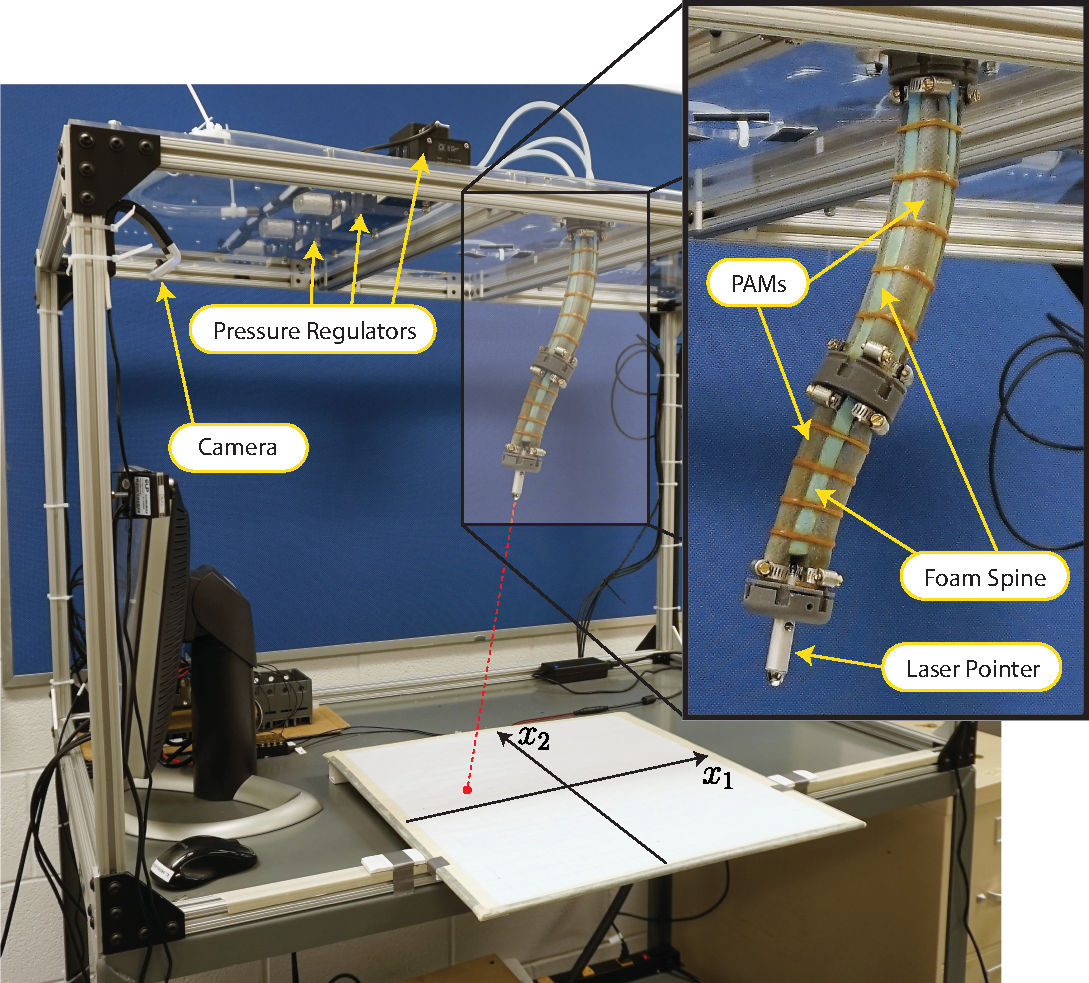
\includegraphics[width=\linewidth]{figures/rig_N_robot_smaller.pdf}
    \caption{The soft robot consists of two bending segments with a laser pointer attached to the end effector. A set of three pressure regulators is used to control the pressure inside of the pneumatic actuators (PAMs), and a camera is used to track the position of the laser dot.}
    \label{fig:rig}
    \vspace*{-0.5cm}
\end{figure}

%% SUBS: NOISE CHARACTERIZATION
\subsection{Characterization of Stochastic Behavior}
\label{sec:noise}

% An input-output system is said to exhibit \emph{stochastic} behavior if identical inputs sometimes produce different outputs.
Most mechanical systems demonstrate stochastic behavior (i.e. when an identical input and state produces a different output) to some extent.
Stochastic behavior is particularly problematic for pneumatic pressure regulators, which can limit the precision of pneumatically driven soft robotic systems
and undermine the predictive capability of models.

We quantified the stochastic behavior of our soft robot system by observing the variations in output from period-to-period under sinusoidal inputs to the three actuators of the form
\begin{align} 
    u[k] &= \begin{bmatrix} 6 \sin ( \frac{2 \pi}{T} k T_s ) + 3 \vspace{5pt} \\ 
    6 \sin ( \frac{2 \pi}{T} k T_s - \frac{T}{3} ) + 3 \vspace{5pt} \\ 
    6 \sin ( \frac{2 \pi}{T} k T_s  - \frac{2T}{3}) + 3\end{bmatrix}
    \label{eq:unoise}
\end{align}
for periods of $T = 6,7,8,9,10,11,12$ seconds and a sampling time of $T_s = 0.1$ seconds with a zero-order-hold between samples. 
Under these inputs, the laser dot traces out a circle with some variability in the trajectory over each period.
In Fig.~\ref{fig:noise} the trajectories over 210 periods are superimposed along with the average over all trials.
Nearly all of the observed points fell within 1 cm of the mean trajectory.
Given this inherent stochasticity of our soft robotic system, we expect only to be able to control the output to within $\approx 1$ cm of a desired trajectory.

%% FIG: Noise inherent to the system
\begin{figure}
    \centering
    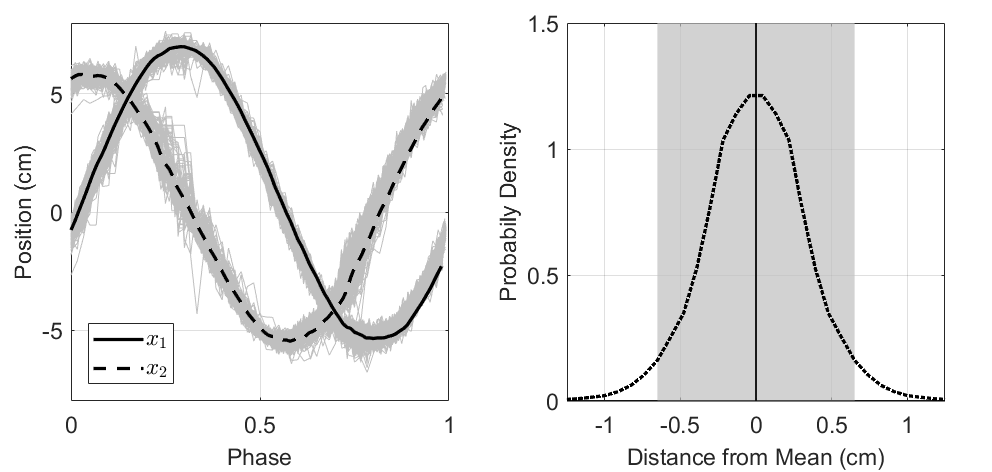
\includegraphics[width=\linewidth]{figures/noise.png}
    \caption{The left plot shows the average response of the system over a single period when the sinusoidal inputs of varying frequencies described by \eqref{eq:unoise} are applied. All of the particular responses are subimposed in light grey.
    The right plot shows the distribution of trajectories about the mean, with all distances within two standard deviations highlighted in grey. The width of the distribution illustrates how for the soft robot system identical inputs can produce outputs that vary by up to 2 cm.}
    \label{fig:noise}
    \vspace*{-0.5cm}
\end{figure}

%% SUBS: DATA COLLECTION
\subsection{Data Collection and Model Identification}
\label{sec:datacollection}

% How data was collected
To construct a model, we ran the system through $16$ trials each lasting approximately $20$ minutes.
A randomized input was applied during each trial to generate a representative sampling of the system's behavior over its entire operating range.
To ensure randomization, a matrix, $\Upsilon \in [0,10]^{3\times 1000}$, of uniformly distributed random numbers between zero and ten was generated to be used as an input lookup table.
Each control input was smoothly varied between elements in consecutive columns of the table over a transition period $T_u$, with a time offset of $T_u / 3$ between each of the three control signals
\begin{align}
    u_i (t) &= \frac{(\Upsilon_{i,k+1} - \Upsilon_{i,k})}{T_u} \left( t + \frac{(i-1) T_u}{3} \right) + \Upsilon_{i,k}
    \label{eq:input}
\end{align}
where $k = \text{floor}\left( {t} / {T_u} \right)$ is the current index into the lookup table at time $t$. 
The transition period $T_u$ varied from $5$ seconds to $10$ seconds between trials.
After collection, the data was uniformly sampled with period $T_s = 0.1$ seconds.

% Models were build from this data
Two models were fit from the data: a Koopman model, and a linear state space model.
The linear state-space model provides a baseline for comparison and was identified from the same data as the Koopman model using the MATLAB System Identification Toolbox \cite{MATLAB:2017}.
This model is a four dimensional linear state-space model expressed in observer canonical form.
The Koopman model was identified via the method described in Section \ref{sec:sysid} on a set of $191,000$ snapshot pairs $\{ a[k] , b[k] \}$ that incorporate a single delay $d = 1$:
\begin{align}
    a[k] &= \begin{bmatrix} x[k]^\top & x[k-1]^\top & u[k-1]^\top \end{bmatrix}^\top \\
    b[k] &= \begin{bmatrix} \left( \phi_{T_s} (x[k]) + \sigma[k] \right)^\top & x[k]^\top & u[k]^\top \end{bmatrix}^\top,
\end{align}
and using the $N=330$ dimensional set of basis functions consisting of all monomials of maximum degree 4.
To find the sparsest acceptable matrix representation of the Koopman operator, equation \eqref{eq:lasso} was solved for ${ \lambda = 0,1,2, ... ,50 }$.
Predictions from the resulting models were evaluated against a subset of the training data, with the error quantified as the average Euclidean distance between the prediction and actual trajectory at each point, normalized by dividing by the average Euclidean distance between the actual trajectory and zero.
Fig.~\ref{fig:lasso} shows that as $\lambda$ increases so does this error, but the density of the $\hat{A}$ matrix of the lifted linear model decreases.
The model chosen is the one that minimizes both density and prediction error, which results in an $\hat{A}$ matrix with $70 \%$ of its entries equal to zero.

%% FIG: MODEL VS. WEIGHT OF L1 PENALTY (LASSO)
\begin{figure}
    \centering
    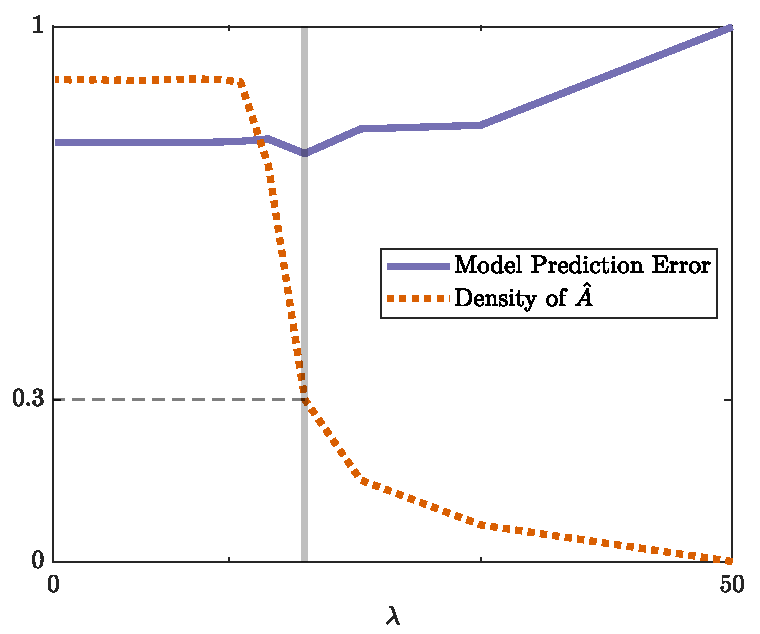
\includegraphics[width=\linewidth]{figures/lasso_v2.pdf}
    \caption{As $\lambda$ (the weight of the $L^1$ penalty term in \eqref{eq:lasso}) increases, the density of the lifted system matrix $\hat{A}$ decreases.
    The model generated by solving \eqref{eq:lasso} with the $\lambda$ valued designated by the vertical grey bar has lower error and a sparser $\hat{A}$ matrix than the least-squares solution to \eqref{eq:koopGamma}, which occurs at $\lambda = 0$.}
    \label{fig:lasso}
    % \vspace*{-0.25cm}
\end{figure}



%% SUBS: PREDICTOR COMPARISON
\subsection{Experiment 1: Model Prediction Comparison}
\label{sec:predict}

The accuracy of the predictions generated by each of the two models were evaluated by comparing them to the actual behavior of the system under the sinusoidal inputs defined in \eqref{eq:unoise}.
The model responses were simulated over a time horizon of $2.5$ seconds given the same initial condition and input as the real system.
The results of this comparison are summarized by Fig. \ref{fig:predict} and Table \ref{tab:predict}. 
They illustrate that the Koopman model predictions are more accurate over the time horizon.

%% FIGURE: Linear vs. Koopman model predictions
\begin{figure}
    \centering
    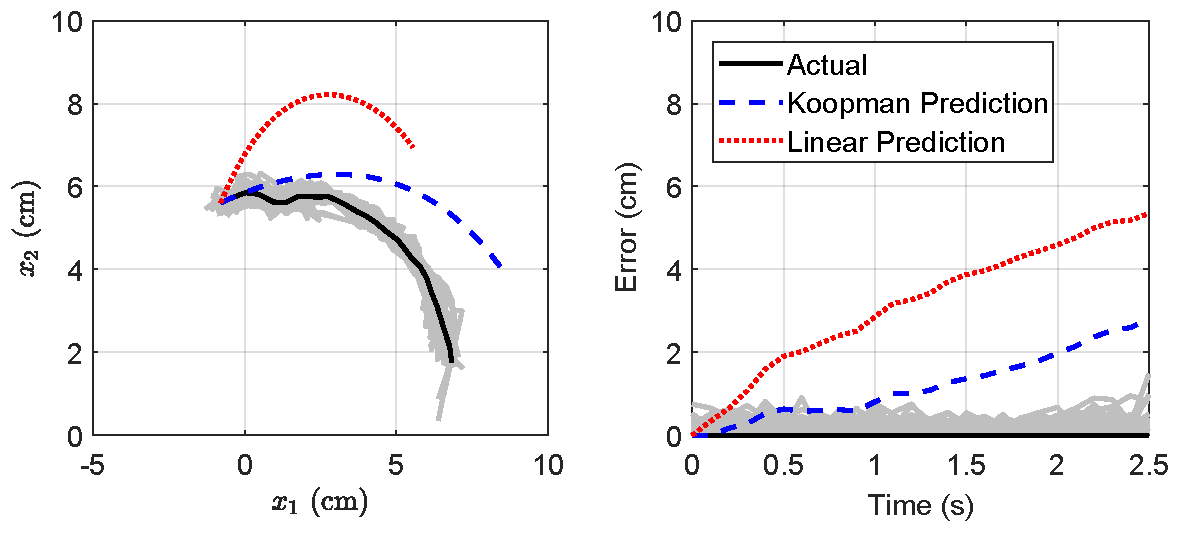
\includegraphics[width=\linewidth]{figures/predictionComparison_v5.pdf}
    \caption{The (average) actual response and the model predictions for the robot over a 2.5 second horizon with the sinusoidal inputs described in \eqref{eq:unoise} with period $T = 10$ seconds applied. The left plot shows the actual trajectory of the laser dot along with model predictions. The error displayed on the right plot is defined as the Euclidean distance between the predicted laser dot position and the actual position at each point in time. The prediction error is smaller for the Koopman model over the entire horizon.}
    \label{fig:predict}
    % \vspace*{-0.5cm}
\end{figure}


%% TABLE: Prediction Comparison
\begin{table}
    \rowcolors{2}{white}{gray!25}
    \setlength\tabcolsep{5pt} % default value: 6pt
    \centering
    \caption{Average Prediction Error Over 2.5 second Horizon (cm)}
    \begin{tabular}{|c|c|c|c|c|c|c|c|c|}
        \hline
        \rowcolor{white} 
        & \multicolumn{7}{c |}{\textbf{Period of Sinusoidal Inputs (seconds)}} & \\
        \cline{2-4} \rowcolor{white}
        \multirow{-2}{*}{\textbf{Model}} & 6 & 7 & 8 & 9 & 10 & 11 & 12 &\multirow{-2}{*}{\textbf{Avg.}} \\
        \hline
        % RESULTS FOR ROBOT A
        Koopman &  2.21  &  2.78 &  1.35  &  1.53  &  1.21 & 0.66 & 1.41 & 1.59 \\
        Linear S.S.  &  4.64  &  4.54  &  3.94 &  3.56  & 3.15 & 2.72 & 2.83 & 3.63 \\
        % Ham.-Weiner &  7.0  &  4.5  &  6.9  &  3.0  &  2.3  &  3.1 & 4.5 & 2.0 \\
        % \multirow{-5}{*}{\cellcolor{white} \rotatebox[origin=c]{90}{\textbf{Robot A}}}
        % NLARX       &  5.0  &  3.0 &  12.0  &  3.8  &  2.1  &  2.8 & 4.8 & 3.7 \\
        \hline
        % % RESULTS FOR ROBOT B
        % \cellcolor{white} & Koopman & & & & & & & & \\
        % \cellcolor{white} & Neural Net & & & & & & & & \\
        % \cellcolor{white} & State Space & & & & & & & & \\
        % \cellcolor{white} & Ham.-Weiner & & & & & & & & \\
        % \multirow{-5}{*}{\cellcolor{white} \rotatebox[origin=c]{90}{\textbf{Robot B}}}
        % & NLARX & & & & & & & & \\
        % \hline
    \end{tabular}
    \label{tab:predict}
\end{table}






%% SUBS: Description of the controllers and tracing task
\subsection{Experiment 2: Model-Based Control Comparison}
\label{sec:mpcexp}

%% FIGURE: Visual results
\begin{figure*}
    \centering
    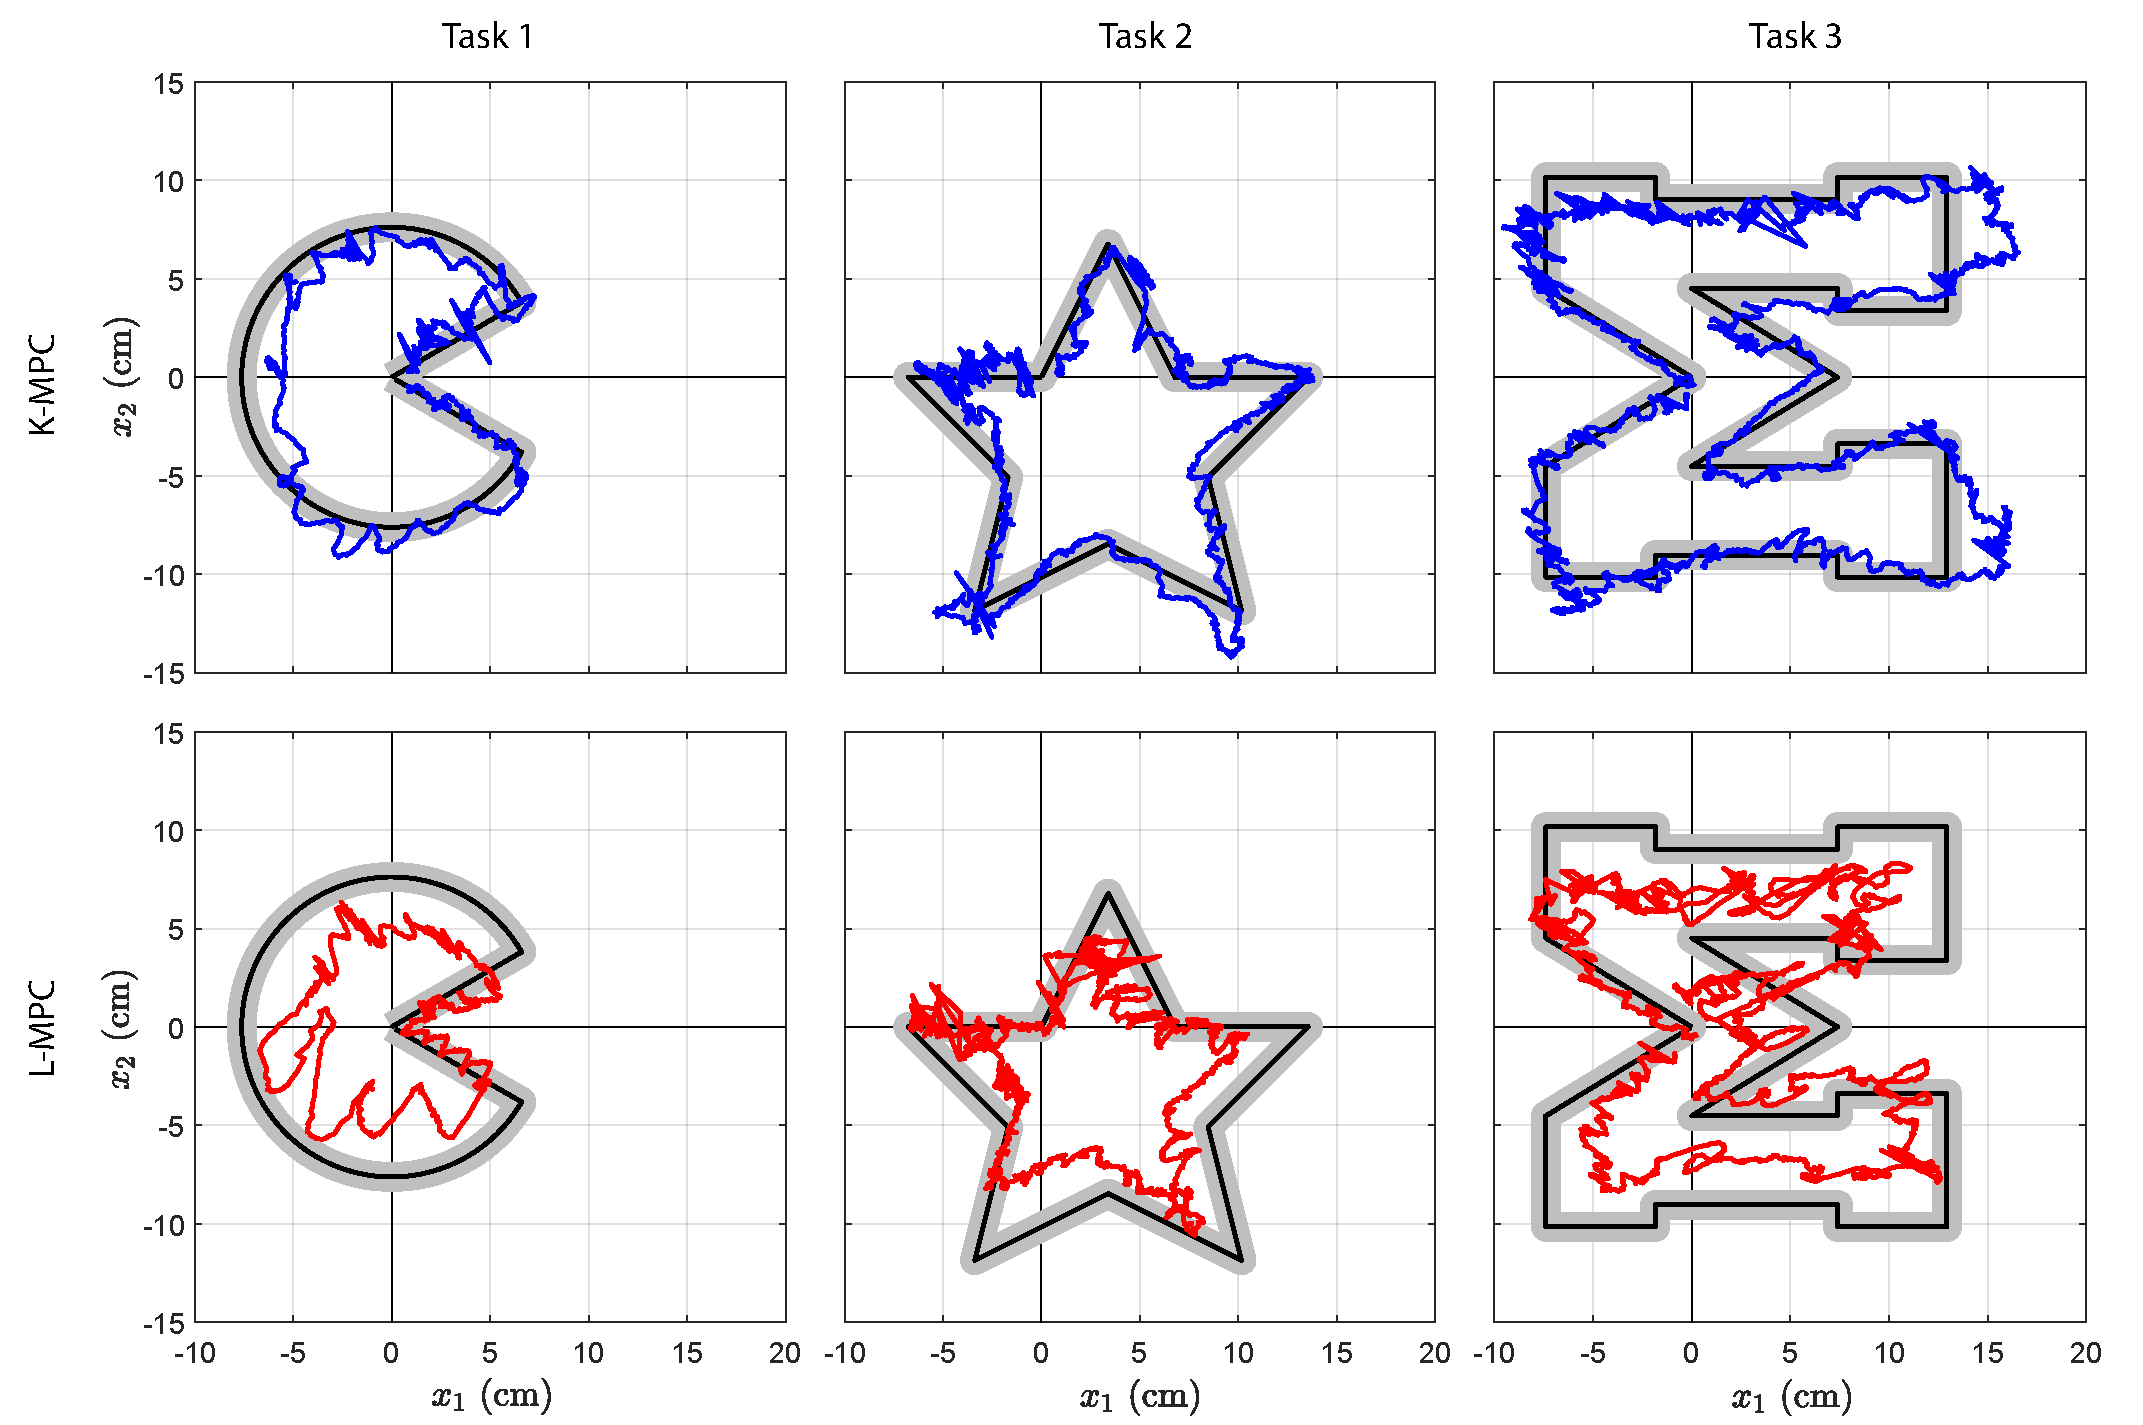
\includegraphics[width=\linewidth]{figures/results_edited_wblue.pdf}
    \caption{The results of the K-MPC controller (row 1, blue) and the L-MPC controller (row 2, red) in performing trajectory following tasks 1-3. The reference trajectory for each task is subimposed in black as well as a grey buffer with width equal to two standard deviations of the noise probability density shown in Fig. \ref{fig:noise}.}
    \label{fig:results}
\end{figure*}


%% Description of compared controllers
The two identified models were each used to build a model predictive controller which solves an optimization problem in the form of \eqref{eq:mpc} at each time step.
We refer to the two controllers by the abbreviations K-MPC for the one based on the Koopman model, and L-MPC for the one based on the linear state-space model. 
%Or: We use the abbreviation K-MPC to refer to the controller based on the Koopman model and L-MPC for the controller based on the linear state-space model.  
Both model predictive controllers run in closed-loop at $10$ Hz, feature an MPC horizon of 2.5 seconds ($N_h = 25$), and a cost function that penalizes deviations from a reference trajectory $r[k]$ over the horizon with both a running and terminal cost:
\begin{align}
    \text{Cost} &= 100 \left( y[N_h] - r[N_h] \right)^2 + \sum_{i=0}^{N_h - 1} 0.1 \left( y[i] - r[i] \right)^2
\end{align}
In the K-MPC case, $y[i] = C z[i]$, where $C$ is defined as in \eqref{eq:C}.
In the L-MPC case, $y[i] = C_L x_L[i]$ where $x_L$ is the four dimensional system state and $C_L$ is the projection matrix that isolates the states describing the current laser dot coordinates. 

% The optimization problem for each controller also featured a convex constraint to limit the rate at which the control inputs could change over time... 

% task
The performance of the controllers was assessed with respect to a set of three trajectory following tasks.
Each task was to follow a reference trajectory as it traced out one of the following shapes over a certain amount of time:
\begin{enumerate}
    \item Pacman (90 seconds)
    \item Star (180 seconds)
    \item Block $\Sigma$ (300 seconds)
\end{enumerate}
The error for each trial was quantified as the Euclidean distance from the reference trajectory at each time step over the length of the trial.

The performances of the K-MPC and L-MPC controllers at Tasks 1, 2, and 3 are shown visually in Fig. \ref{fig:results}, and the error is quantified in Table \ref{tab:RMSE}.
In both tasks the K-MPC controller achieved better performance, exhibiting an average tracking error of 1.26~cm compared to the L-MPC controller's average error of 2.45~cm.
This amounts to an average error roughly $25\%$ larger than than the maximum magnitude of observed noise (see Fig. \ref{fig:noise})
% The magnitude of this error was larger than the maximum magnitude of observed noise (see Fig. \ref{fig:noise}), but only by about one quarter of a centimeter, or $1 \%$ of the total range of motion observed. 



%% TABLE: RMSE results table
\begin{table}
    \rowcolors{2}{white}{gray!25}
    \setlength\tabcolsep{5pt} % default value: 6pt
    \centering
    \caption{Average Error in Trajectory Following Tasks (cm)}
    \begin{tabular}{|c|c|c|c|c|c|}
        \hline
        \rowcolor{white} 
        & \multicolumn{3}{c |}{\textbf{Task}} & & \textbf{Std.} \\
        \cline{2-4} \rowcolor{white}
        \multirow{-2}{*}{\textbf{Controller}} & $1$ & $2$ & $3$ & \multirow{-2}{*}{\textbf{Avg.}} & \textbf{Dev.} \\
        \hline
        % RESULTS FOR ROBOT A
        K-MPC &  1.25  &  1.19 &  1.34  &  1.26  &  0.07  \\
        L-MPC  &  2.21  &  2.34  &  2.73 &  2.45  &  0.31   \\
        % Ham.-Weiner &  7.0  &  4.5  &  6.9  &  3.0  &  2.3  &  3.1 & 4.5 & 2.0 \\
        % \multirow{-5}{*}{\cellcolor{white} \rotatebox[origin=c]{90}{\textbf{Robot A}}}
        % NLARX       &  5.0  &  3.0 &  12.0  &  3.8  &  2.1  &  2.8 & 4.8 & 3.7 \\
        \hline
        % % RESULTS FOR ROBOT B
        % \cellcolor{white} & Koopman & & & & & & & & \\
        % \cellcolor{white} & Neural Net & & & & & & & & \\
        % \cellcolor{white} & State Space & & & & & & & & \\
        % \cellcolor{white} & Ham.-Weiner & & & & & & & & \\
        % \multirow{-5}{*}{\cellcolor{white} \rotatebox[origin=c]{90}{\textbf{Robot B}}}
        % & NLARX & & & & & & & & \\
        % \hline
    \end{tabular}
    \label{tab:RMSE}
\end{table}
